\section{Support Vector Machines}

\subsection{Linear support vector machines}
Figure~\ref{fig:svm-l} shows the results of a single support vector machine with a linear kernel function. 

A first observation os that the number of support vector machines has a very high influence on the speed of the evaluation through MPC. A very interesting observation is that the tree-based classifier do not perform worse that the one-against-all model. Indeed, the order of the tree-based is very important as it can make the tree-based model perform better or worse than one-against-all models. In this sense, the best tree-based structure does perform better and has a faster evaluation through MPC as it comprises one SVM less.

Secondly, as we can see, the results are quite satisfying. The accuracy is high, nevertheless, the results must be nuanced. Indeed, the accuracy doesn't take into account the initial distribution of the classes. This is very important if the initial distribution of a class is not uniform. Let us imagine a data-set where a same class represents a vast majority of the instances -- let's say 90\%. If we imagine a classifier that classifies this class very well and the other classes in a totally not satisfying way, the accuracy would be very high as the main class would weigh a lots in it. This would not be the case with Matthew's correlation coefficient, which takes into account the ratios between the classes. A lower Matthew's correlation coefficient may indicate some classes that are not making a big part of the data and thus weigh not so much on the accuracy, but are still often miscalssified.

\begin{figure}
        \begin{subfigure}[b]{1\textwidth}  
            \centering 
            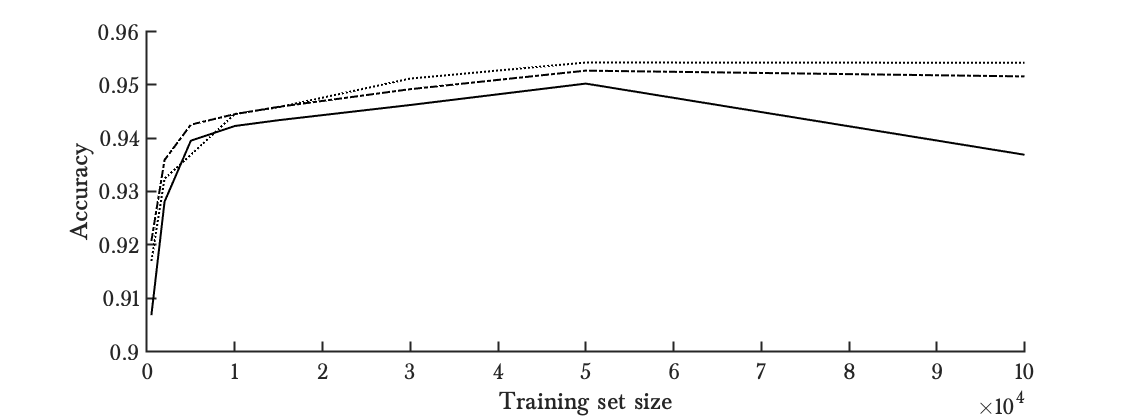
\includegraphics[width=.98\textwidth]{parts/chap-4/img-svm/lin-svm-1.png}
            \caption{Mean Accuracy on the test set.} 
        \end{subfigure}
        \vfill
        \begin{subfigure}[b]{1\textwidth}   
            \centering 
            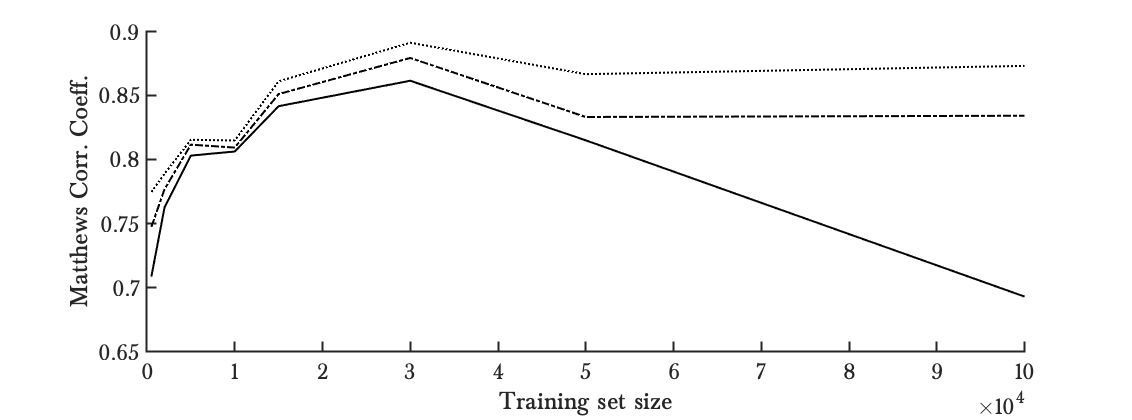
\includegraphics[width=.98\textwidth]{parts/chap-4/img-svm/lin-svm-2.png}
            \caption{Mean Mathews correlation coefficient.} 
        \end{subfigure}
        \vfill
        \begin{subfigure}[b]{1\textwidth}   
            \centering 
            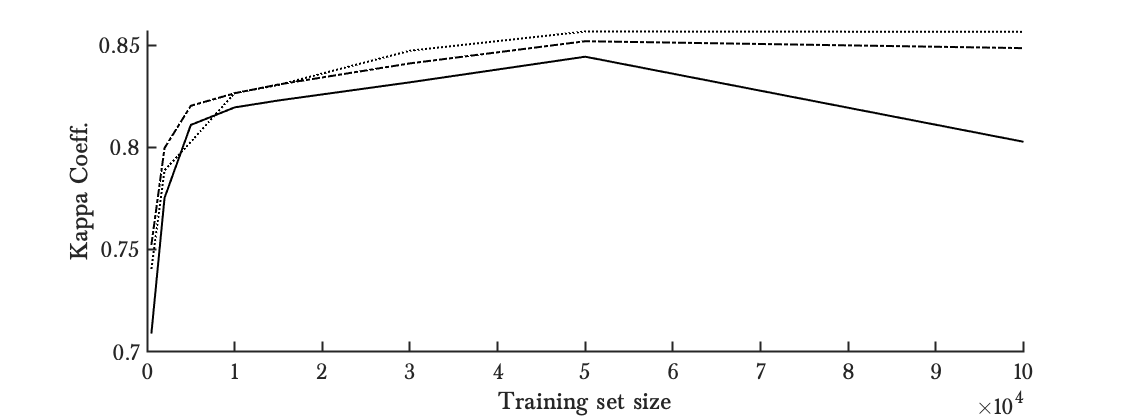
\includegraphics[width=.98\textwidth]{parts/chap-4/img-svm/lin-svm-3.png}
            \caption{Mean Cohen's kappa coefficient.} 
        \end{subfigure}
        \caption{Evaluation of three different models in function of the training set size. The one-against-all (or parallel) model is in dash-dotted line, the tree-bases model (or parallel) are the plain and dotted line. For the plain line, the order of the SVMs is \{Normal, DoS, Prob, R2L, U2R\} and the dotted line is \{Probe, U2R, R2L, DoS, Normal\}. Every result is the mean of 5 different experiments with different training and test set.}
        \label{fig:svm-l}
\end{figure}

Cohen's kappa score indicates something similar. A high value Indeed, We therefore must have a more detailed look at the results (tables~\ref{tab:svm-l-0}, \ref{tab:svm-l-1} and \ref{tab:svm-l-2}). 

A first observation is that the very low number of U2R and in a lesser manner of R2L instances in the training set size lead to a not very satisfying classification. The data of this class not being able to be classified well, this leads to a low MCC coefficient. However, the wrong results are mainly attributed to the normal class. This makes sense as the low number of instances makes the classifier not really able to generalize the properties of this class, not being able to recognize it well and thus unable to distinguish from a normal instance. However, the fact that the false negatives being mainly attributed to the normal class and not randomly assigned to the other classes explains the high kappa coefficient. This example justifies the use of those two coefficients together as they are, in this example complementary. Not much can be done to solve this issue except massively augmenting the presence of the U2R --- and in a lesser way R2L --- presence in the training data-set. This low result is also to be nuanced as their scarce appearance is also an indication for their low frequency in real-life cases. We can thus conclude that the model doesn't detect much of these attacks, but hopefully they are scarce. 

A second observation is the very low kappa coefficient for the normal class and the details indicate that the normal instance identified as attacks are proportionally distributed among the other classes, which translates into a much higher Matthews correlation coefficient (MCC). In other words, misclassified normal classes don't tend to be identified as one class specifically above another.

A third observation is that the results get better with the training size, which is an expected result in machine learning. However, for small training sizes the one-against-all model performs better than both tree-based models. This is to be nuanced du to the small training size which can lead to a much higher variance in the results. However, after some time, one of the two tree-based models preform slightly better that the one-against-all model. As said before, this is a very insteresting observation as these models demand one less SVM for training and evaluation, which is one of the key performances for us. Also, the MCC starts to drop after some time. This is due to the fact that it is much more sensitive to missclassified values than well classified values, and this difference tends to increase with the test size.

Overall, they are two key observations The fist one is that one-against-all models are not better than tree-based models, it just depends on the order of the tree. The second one is that training sets bigger than 30,000 don't make a lot of difference anymore. This facts certainly matter for the evaluation, but not much for the evaluation as linear SVMs only depend on the feature size in their primal form. However, this will have impact when the evaluation is done in the dual, e.g. RBF-SVMs -- but this is a talk for later.

\begin{table}[ht!]
    \centering
    \begin{tabularx}{\textwidth}{lcccccc}
    \hlineI
    Model & Normal & Probe & Dos & R2L & U2R & Total \\ \hlineI
    \textbf{Tree 1} with $n=2000$ & & & & & &\\
    Accuracy [\%] & 87.67 & 96.36 & 96.13 & 94.30 & 46.67 & 92.81\\ 
    MCC & 86.34 & 95.69 & 91.36 & 72.66 & 35.29 & 70.86\\ 
    Kappa & 29.17 & 42.85 & 41.90 & 92.27 & 99.66 & 70.88\\ \hline
    Obs. Normal  & 2630 & 38 & 175 & 145 & 12 & \\ 
    Obs. Probe  & 56 & 2172 & 20 & 5 & 0 & \\ 
    Obs. DoS  & 63 & 17 & 2167 & 6 & 1 & \\ 
    Obs. R2L  & 13 & 0 & 0 & 215 & 0 & \\ 
    Obs. U2R  & 0 & 0 & 0 & 5 & 4 & \\  \hlineI
    
    \textbf{Tree 2} with $n=2000$ & & & & & &\\
    Accuracy [\%] & 90.55 & 96.22 & 95.37 & 91.93 & 44.44 & 91.96\\ 
    MCC & 87.67 & 96.01 & 91.27 & 78.55 & 34.90 & 77.45\\ 
    Kappa & 27.41 & 43.01 & 42.32 & 93.14 & 99.70 & 74.04\\  \hline 
    Obs. Normal  & 2717 & 27 & 161 & 86 & 9 & \\ 
    Obs. Probe  & 65 & 2169 & 17 & 2 & 0 & \\ 
    Obs. DoS  & 86 & 14 & 2150 & 4 & 0 & \\ 
    Obs. R2L  & 17 & 1 & 0 & 210 & 1 & \\ 
    Obs. U2R  & 0 & 0 & 0 & 5 & 4 & \\ \hlineI
    
    \textbf{O-A-A} with $n=2000$ & & & & & &\\
    Accuracy [\%] & 91.70 & 95.41 & 93.40 & 92.46 & 44.44 & 92.07\\ 
    MCC & 86.90 & 95.87 & 90.26 & 79.28 & 42.14 & 74.74\\ 
    Kappa & 26.47 & 43.43 & 43.22 & 93.16 & 99.75 & 75.22\\  \hline
    Obs. Normal  & 2751 & 11 & 149 & 83 & 6 & \\ 
    Obs. Probe  & 88 & 2151 & 14 & 1 & 0 & \\ 
    Obs. DoS  & 127 & 17 & 2105 & 5 & 0 & \\ 
    Obs. R2L  & 17 & 0 & 0 & 211 & 0 & \\ 
    Obs. U2R  & 0 & 0 & 0 & 5 & 4 & \\  \hlineI
    \end{tabularx}
    \caption{Detailed results of the $k$-NN classification algorithm for two different values of the number of neighbours $k$ and for a big and a small training data-set. The accuracy, true positive rate (TP), true negative rate (TN), false positive rate (FP) and false negative rate (FN) are given for each target class.}
    \label{tab:svm-l-0}
\end{table}

\begin{table}[ht!]
    \centering
    \begin{tabularx}{\textwidth}{lcccccc}
    \hlineI
    Model & Normal & Probe & Dos & R2L & U2R & Total \\ \hlineI
    \textbf{Tree 1} with $n=30,000$ & & & & & &\\
    Accuracy [\%] & 91.37 & 97.40 & 96.34 & 94.07 & 73.33 & 94.62\\ 
    MCC & 89.00 & 96.03 & 93.15 & 85.20 & 67.38 & 86.15\\
    Kappa & 27.06 & 42.34 & 42.25 & 93.59 & 99.66 & 83.19\\ \hline
    Obs. Normal  & 2741 & 63 & 136 & 55 & 5 & \\ 
    Obs. Probe  & 53 & 2195 & 2 & 3 & 0 & \\ 
    Obs. DoS  & 76 & 5 & 2171 & 1 & 0 & \\ 
    Obs. R2L  & 13 & 0 & 0 & 213 & 0 & \\ 
    Obs. U2R  & 2 & 0 & 0 & 1 & 9 & \\  \hlineI
    
    \textbf{Tree 2} with $n=30,000$ & & & & & &\\
    Accuracy [\%] & 92.56 & 97.11 & 96.18 & 93.27 & 66.67 & 95.12\\ 
    MCC & 89.84 & 96.82 & 92.39 & 87.16 & 73.46 & 89.12\\ 
    Kappa & 26.35 & 42.70 & 42.14 & 93.79 & 99.72 & 84.74\\ \hline 
    Obs. Normal  & 2777 & 29 & 151 & 42 & 2 & \\ 
    Obs. Probe  & 56 & 2189 & 9 & 0 & 0 & \\ 
    Obs. DoS  & 80 & 6 & 2168 & 0 & 0 & \\ 
    Obs. R2L  & 14 & 1 & 0 & 211 & 0 & \\ 
    Obs. U2R  & 0 & 0 & 0 & 4 & 8 & \\ \hlineI
    
    \textbf{O-A-A} with $n=30,000$ & & & & & &\\
    Accuracy [\%] & 93.03 & 96.67 & 96.53 & 94.60 & 70 & 94.62\\ 
    MCC & 90.13 & 96.84 & 92.81 & 88.31 & 77.52 & 87.93\\ 
    Kappa & 26.07 & 42.96 & 42.05 & 93.78 & 99.72 & 84.12\\ \hline
    Obs. Normal  & 2791 & 18 & 150 & 40 & 1 & \\ 
    Obs. Probe  & 71 & 2179 & 4 & 0 & 0 & \\ 
    Obs. DoS  & 70 & 8 & 2176 & 0 & 0 & \\ 
    Obs. R2L  & 12 & 0 & 0 & 214 & 0 & \\ 
    Obs. U2R  & 0 & 0 & 0 & 3 & 8 &\\ \hlineI
    \end{tabularx}
    \caption{Detailed results of the $k$-NN classification algorithm for two different values of the number of neighbours $k$ and for a big and a small training data-set. The accuracy, true positive rate (TP), true negative rate (TN), false positive rate (FP) and false negative rate (FN) are given for each target class.}
    \label{tab:svm-l-1}
\end{table}
    
\begin{table}[ht!]
    \centering
    \begin{tabularx}{\textwidth}{lcccccc}
    \hlineI
    Model & Normal & Probe & Dos & R2L & U2R & Total \\ \hlineI
    \textbf{Tree 1} $n=100,000$ & & & & & &\\
    Accuracy [\%] & 93.19 & 97.77 & 95.68 & 35.75 & 10.77 & 93.96\\ 
    MCC & 87.08 & 96.69 & 92.77 & 50.96 & 18.95 & 69.29\\ 
    Kappa & 25.33 & 41.94 & 42.19 & 96.34 & 99.79 & 80.28\\ \hline
    Obs. Normal  & 2796 & 48 & 133 & 22 & 1 & \\ 
    Obs. Probe  &48 & 2214 & 2 & 0 & 0 & \\ 
    Obs. DoS  & 91 & 7 & 2167 & 0 & 0 & \\ 
    Obs. R2L  & 123 & 0 & 0 & 69 & 1 & \\ 
    Obs. U2R  & 11 & 0 & 0 & 1 & 1 & \\  \hlineI
    
    \textbf{Tree 2} $n=100,000$ & & & & & &\\
    Accuracy [\%] & 93.51 & 97.35 & 96.74 & 80.41 & 36.92 & 95.41\\ 
    MCC & 90.34 & 97.31 & 92.79 & 82.31 & 54.36 & 87.31\\ 
    Kappa & 25.66 & 42.33 & 41.57 & 95.17 & 99.76 & 85.67\\ \hline
    Obs. Normal  & 2805 & 20 & 150 & 24 & 0 & \\ 
    Obs. Probe  & 49 & 2205 & 11 & 0 & 0 & \\ 
    Obs. DoS  & 67 & 6 & 2191 & 1 & 0 & \\ 
    Obs. R2L  & 37 & 0 & 0 & 155 & 1 & \\ 
    Obs. U2R  & 6 & 0 & 0 & 2 & 5 & \\ \hlineI
    
    \textbf{O-A-A} $n=100,000$ & & & & & &\\
    Accuracy [\%] & 93.39 & 96.97 & 97.58 & 85.49 & 61.54 & 93.96\\ 
    MCC & 90.77 & 97.50 & 93.26 & 83.32 & 71.71 & 83.42\\ 
    Kappa & 25.82 & 42.60 & 41.19 & 94.93 & 99.71 & 84.87\\ \hline
    Obs. Normal  & 2802 & 7 & 164 & 27 & 0 & \\ 
    Obs. Probe  & 67 & 2196 & 2 & 0 & 0 & \\ 
    Obs. DoS  & 45 & 4 & 2210 & 6 & 0 & \\ 
    Obs. R2L  & 27 & 0 & 0 & 165 & 1 & \\ 
    Obs. U2R  & 2 & 0 & 0 & 3 & 8 & \\ \hlineI
    \end{tabularx}
    \caption{Detailed results of the $k$-NN classification algorithm for two different values of the number of neighbours $k$ and for a big and a small training data-set. The accuracy, true positive rate (TP), true negative rate (TN), false positive rate (FP) and false negative rate (FN) are given for each target class.}
    \label{tab:svm-l-2}
\end{table}

\FloatBarrier
\subsubsection{PCA reduction}

\begin{wrapfigure}[17]{r}{0.45\textwidth}
\begin{center}
    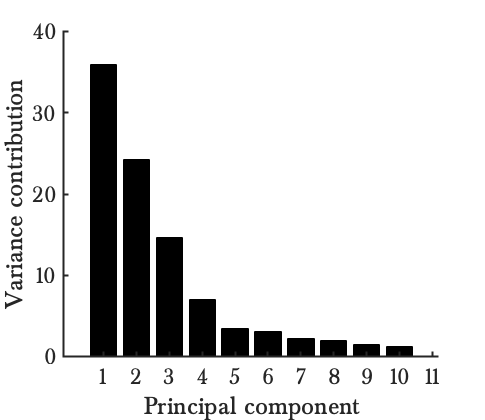
\includegraphics[width=.45\textwidth]{parts/chap-4/img-svm/pca-var.png}
    \caption{Variance participation of the 11 first support vectors.}
    \label{fig:pca-var}
\end{center}
\end{wrapfigure}
Let us now investigate how a principal components decomposition affects the accuracy and allows us to win execution time. The variance contribution of the first principal components is given at figure~\ref{fig:pca-var}. As the variance contribution is not drastically decreasing, this plots indicates us that much of the features are relevant and not so much of it is due to linear combinations of others features. This also suggests by consequence that we will not be able to limit ourselves to a projection into a space of much smaller dimension. The influence of a training for a varying number of principal components kept --- which corresonds to the dimension of the projected space --- is given at figure~\ref{fig:svm-pca}. We thereby conclude that we cannot limit ourselves to 6 features as a elbow rule would suggest, but that we need more of them, e.g. 16. The more detailed results for those both number of PCA kep are given at tables~\ref{tab:pca-1} and \ref{tab:pca-2}. Here again, we can conclude, that there is no significant difference between the tree-based model or the one-againt-all model. 

\begin{figure}[ht!]
        \begin{subfigure}[b]{1\textwidth}  
            \centering 
            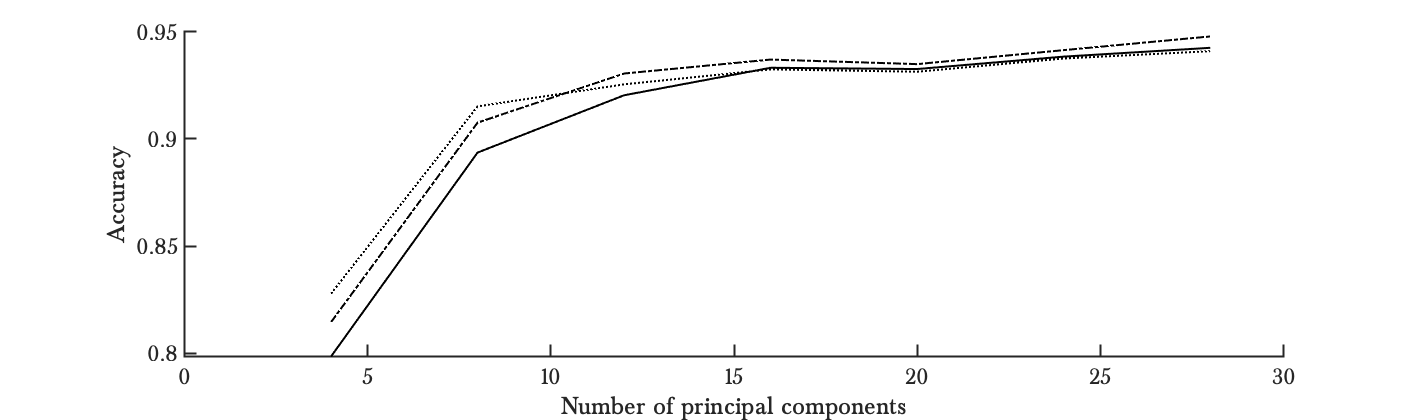
\includegraphics[width=.98\textwidth]{parts/chap-4/img-svm/pca-acc.png}
            \caption{Mean of the accuracy on the test set.} 
        \end{subfigure}
        \vfill
        \begin{subfigure}[b]{1\textwidth}   
            \centering 
            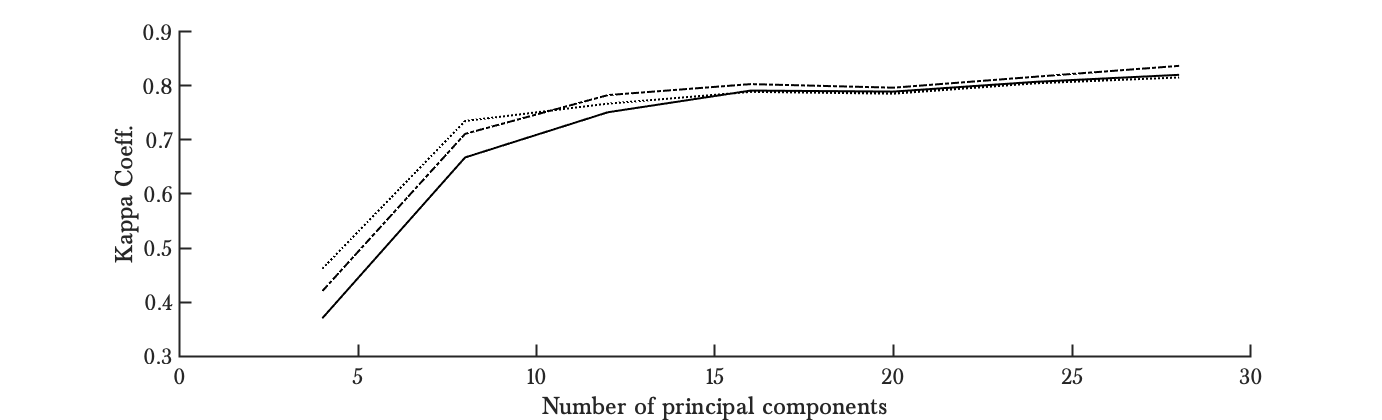
\includegraphics[width=.98\textwidth]{parts/chap-4/img-svm/pca-kappa.png}
            \caption{Mean of Cohen's kappa coefficient.} 
        \end{subfigure}
        \caption{Evaluation of three different models in function of number of principal komponents kept. The one-against-all (or parallel) model is in dash-dotted line, the tree-bases model (or parallel) are the plain and dotted line. For the plain line, the order of the SVMs is \{Normal, DoS, Prob, R2L, U2R\} and the dotted line is \{Probe, U2R, R2L, DoS, Normal\}. Every result is the mean of 5 different experiments with different training and test sets.}
        \label{fig:svm-pca}
\end{figure}

\begin{table}[ht!]
    \centering
    \begin{tabularx}{\textwidth}{lcccccc}
    \hlineI
    Model & Normal & Probe & Dos & R2L & U2R & Total \\ \hlineI
    \textbf{Tree} with $n_{pca}=8$ & & & & & &\\
    Accuracy [\%] & 91.49 & 92.01 & 91.33 & 93.33 & 3.64 & 91.51\\ 
    MCC [\%] & 87.21 & 91.53 & 87.34 & 70.16 & $\emptyset$ & $\emptyset$\\ 
    Kappa [\%] & 26.55 & 43.84 & 43.22 & 93.69 & 99.84 & 71.11\\ \hline
    Obs. Normal & 2745 & 46 & 123 & 86 & 0 & \\ 
    Obs. Probe  &93 & 2089 & 87 & 1 & 0 & \\ 
    Obs. DoS  & 104 & 42 & 2073 & 51 & 0 & \\ 
    Obs. R2L  & 12 & 0 & 0 & 168 & 0 & \\ 
    Obs. U2R  & 5 & 0 & 0 & 6 & 0 & \\  \hlineI
    
    \textbf{O-A-A} with $n_{pca}=8$ & & & & & &\\
    Accuracy [\%] & 87.50 & 91.54 & 94.28 & 95.33 & 12.73 & 90.75 \\ 
    MCC [\%] & 85.62 & 91.02 & 88.42 & 71.14 & 4.13 & 68.07 \\ 
    Kappa [\%] & 29.07 & 43.99 & 41.76 & 93.60 & 98.90 & 71.11 \\  \hline
    Obs. Normal  & 2625 & 50 & 137 & 127 & 61 & \\ 
    Obs. Probe  & 76 & 2078 & 112 & 2 & 1 & \\ 
    Obs. DoS  & 67 & 44 & 2140 & 11 & 9 & \\ 
    Obs. R2L  & 7 & 0 & 0 & 172 & 1 & \\ 
    Obs. U2R  & 2 & 0 & 0 & 8 & 1 & \\ \hlineI
    \end{tabularx}
    \caption{Detailed results of the $k$-NN classification algorithm for two different values of the number of neighbours $k$ and for a big and a small training data-set. The accuracy, true positive rate (TP), true negative rate (TN), false positive rate (FP) and false negative rate (FN) are given for each target class.}
    \label{tab:pca-1}
\end{table}

\begin{table}[ht!]
    \centering
    \begin{tabularx}{\textwidth}{lcccccc}
    \hlineI
    Model & Normal & Probe & Dos & R2L & U2R & Total \\ \hlineI
    \textbf{Tree} with $n_{pca}=16$ & & & & & &\\
    Accuracy [\%] & 91.33 & 94.94 & 94.19 & 96.11 & 33.33 & 93.24\\ 
    MCC & 87.13 & 95.35 & 90.77 & 79.68 & $\emptyset$ & $\emptyset$\\ 
    Kappa & 26.76 & 43.51 & 42.83 & 93.25 & 99.62 & 78.86 \\  \hline
    Obs. Normal  & 2740 & 12 & 150 & 89 & 8 & \\ 
    Obs. Probe  &98 & 2142 & 16 & 1 & 0 & \\ 
    Obs. DoS  & 100 & 22 & 2125 & 8 & 1 & \\ 
    Obs. R2L  & 8 & 0 & 0 & 208 & 0 & \\ 
    Obs. U2R  & 6 & 0 & 0 & 4 & 5 & \\   \hlineI
    
    \textbf{O-A-A} with $n_{pca}=16$ & & & & & &\\
    Accuracy [\%] & 91.11 & 95.55 & 95.63 & 95.09 & 18.67 & 93.31\\ 
    MCC & 88.16 & 95.62 & 91.18 & 80.59 & 25.99 & 76.31\\ 
    Kappa & 27.08 & 43.23 & 42.09 & 93.42 & 99.74 & 80.29\\  \hline
    Obs. Normal  & 2733 & 24 & 162 & 80 & 1 & \\ 
    Obs. Probe  & 72 & 2156 & 26 & 3 & 0 & \\ 
    Obs. DoS  & 80 & 15 & 2157 & 2 & 1 & \\ 
    Obs. R2L  & 10 & 0 & 1 & 205 & 0 & \\ 
    Obs. U2R  & 6 & 0 & 0 & 6 & 3 & \\  \hlineI
    \end{tabularx}
    \caption{Detailed results of the $k$-NN classification algorithm for two different values of the number of neighbours $k$ and for a big and a small training data-set. The accuracy, true positive rate (TP), true negative rate (TN), false positive rate (FP) and false negative rate (FN) are given for each target class.}
    \label{tab:pca-2}
\end{table}

An interesting thing with PCA is to think if we could only perform one of the operations (PCA or SVM) and do the other one in clear. Lets us investigate the consequences:
\begin{itemize}
    \item \textbf{Hidden PCA - Clear SVM.} The first idea of doing the PCA tranfsformation in MPC and evaluating the SVM in clear is not very good. It is very naïve to think that PCA destructs the data in such a way that the transformed feature lose much of their information. By transforming using a principal component analysis, we aim at the exact opposite which is to keep as much variance possible, thus as much as information as possible. By looking hereabove at the results of the classifier after the PCA reduction, we notice that the PCA reduction does approach the same classification performance as without. Using clear SVM has also the results that everyone that participates to the evaluation of the transformed data-point can see its classification result. 
    
    The clear SVM evaluation should therefore be limited to the strict minimum parties, i.e. the model owner sending the SVM-model to the query owner which then performs the classification on its own. In this way, his data-point is always hidden, but the model owner reveals a part of his model. However, this model part is unusable in itself as it needs the PCA transformation, which is still hidden.

    The other possibility to keep the whole model (PCA and SVM) hidden is that the query owner sends its query after PCA to the model owner for him to perform the classification. The owner of the model data, once he knows the transformation of the query point, cannot recover it completely. One can notice than computing the inverse of the PCA reduction will lead to some noisy pre-image in the sense that the pre-image is a not a single data-point but a distribution with variance corresponding to the variance list with the PCA transformation. This ressembles to differential privacy, but we will not go further into this direction. To summarize, this will of course reveal the final output (the eventual attack and its type), but somewhat hide the features about the query (e.g. duration or status of the connection). This justifies the preference for the model owner sending the SVM-model to the query owner which then performs the classification on its own. In this scenario, the owner however keeps all its model protected.
    
    Finally, one should add that this whole idea of computing the principal component analysis in MPC and then the SVM in clear is computationally doubtful as the MPC-based PCA-transformation of the query point demands $\mathcal{O}\left(n_{pca}d\right)$ MPC multiplication operations where $d$ is the feature size and $n_{pca}$ the number of principal components kept, here more than 6 for reasonnable performance. Evaluating multi-class support vector machines without PCA and totally hidden has a complexity of $\mathcal{O}(n_{svm}d)$ MPC multiplication operations where $n_{svm}$ is the number of SVMs in the multi-class model, here 4 or 5 depending on which model structure is used. Once the PCA transformation is complete, you still have to add the designation of a winner between the different binary SVMs output which takes $\mathcal{O}(n_{svm})$ MPC comparison operations which are known to be more expensive than multiplications. The question is if the fact that $n_{pca} > n_{svm}$ is compensated by the hidden election of a winner.
    
    \item \textbf{Clear PCA - Hidden SVM.}
    This alternative has the same property as before, the model is still partially hidden. Furthermore, the hidden evaluation of the SVM guarantees the privacy of the final classification output. Conversely as before, the question of whom evaluates the PCA decomposition has only one possibility, the query owner as the opposite would reveal the initial feature vector to someone else and loose all the privacy of the queried point.
    
    The first question if we reveal the PCA components is what information is revealed. Well, not much as this is the result of the sole diagonalization of the correlation matrix of the model owner's initial data-points. The correlation matrix instrisically reveals the linear relations between different features. This would harshly reveal anything about the original data-points as this relation is computed amongst ideally several thousands of points from all classes alltogether. Furthermore, this correlation matrix is diagonalized and the sole first components are kept, revealing in a certain sense the sole important relations. With the hypothesis that each class has different subjacent relations and thus different principal components \noteH{maybe test this hypothesis ?}, an attacker could --- but this is going quite far --- deduce which classes were present in the model owner original data-set and thus deduce to which attack he is subject to, or at least detected. However, the exact nature of the original individual data-points remains secret and so does the queried data-point as it never leaves its owner in clear form.
    
    The advantage of this method is that performing an hidden SVM with pre-computed PCA reduction reduces the complexity from $\mathcal{O}(n_{svm}d)$ to $\mathcal{O}(n_{svm}n_{pca})$ and in the practice of a factor between 2 and 4. However, the designation of the winning SVM remains $\mathcal{O}(n_{svm})$.
    
    \item \textbf{No PCA - Clear SVM.} In this case, the query owner recieves the whole model from the model owner. Of course, not much here is still hidden. In fact, all the model is clear an can be used by anybody who recieves it and there is no need at all for MPC techniques. However linear SVM have the big advantage against the other ones, using kernel trick, that it doesn't need the dual to be computed. This means that instead of sending the $\alpha_i$ with their corresponding support vectors $x_i$ and targets $l_i$ (which will be of course a huge breach of privacy-friendliness), one can just send the weights vector $w$ (and the bias $b$), which reveals much less information about the model. The exact relation between the weights and the support vectors is 
    \begin{equation}
        w = \sum_{\forall i}\alpha_i l_i x_i
    \end{equation}
    The bias stays the same. The computation of the wieghts is of course a very big compression of the support vectors and destroys the information they contain. In this sense, a totally clear model could be an option, depending on the choices of the model owner. Considering the execution speed, this has no competitor among the model we test as avoiding the use of MPC leads to drastic speed evaluations. A drawback however, that has less to do with privacy-friendliness but is still relevant is the loss of control the owner of the model gets with this method. Indeed, the big advantage of using MPC on a significant part of the model is that the other celar parts of the model are unusable without the MPC-part, whose parameters are never revealed. In this sense, the owner of the data still has a full control as he is the sole who can ultimately decide whether or not his model can be used. Once all is in clear, this property disappears and there is no more secure lock against the proliferation of the models use without its consent. This can be relevant for commercial uses for example\footnote{Besides, this raises an interesting question on how to secure software against illegal proliferation and use. Instead of using license keys, why just not performing a very small, but essential task in MPC without which the program could possibly work (in an information-theoretic scheme). In this sense, the owner is sure that only identified users --- which he can control at each instant --- are allowed to use the program. This of course would need to rest on a permanent internet connection (which is nowadays less a problem, more and more smartphone apps are requiring a permanent internet connection) and avoiding the MPC task being cracked and substituted by local version. This is a totally out of the scope of my thesis, but I believe the question to be interesting. Of course, this idea could also be used without MPC and just data snet in ean encrypted form, but this would not be privacy-friendly for the user. Another question would also be, who be the third party to avoid a malicious majority, the first party being the user and the second the company. The third party would be a party that has no interest in working with the user and thus cracking the program nor with the firm issuing the program revealing the user's data. This could be replaced by homomorphic encryption to avoid the use a of third party but is computationally more \noteH{?} costly.}.
\end{itemize}

\FloatBarrier
\subsubsection{$\chi^2$-reduction}
Where the PCA decomposition is the same for all binary SVM, the $\chi^2$ feature selection allows us to select the most relevant features for each SVM. This allows us for a more specifically pre-processed classifiers. Here, the big advantage is a reduction of complexity from $\mathcal{O}(n_{svm}d)$ to $\mathcal{O}(n_{svm}n_{\chi^2})$ where $n_{\chi^2}$ s the number of features kept. In our case, the reduction results in a reduction of 30\% of the feature inputs and thus an expected similar speed win. Table~\ref{tab:svm-l-chi2} shows the execution of the three models and we can see that there is no significant loss in accuracy compared to the other models. However, the training of a $\chi^2$ selection is much slower because it asks to train $d$ support vector machines per binary classification instead of one. However, as we said, the evaluation time got a speed increase. In other words, we won at evaluating time at the cost of training time. The good part is that the training is only done once normally, at the contrary of the MPC-evaluation which proportionally much more coslty. This is a clear example of the training-evaluating trade-off we try to take advantage of.

\begin{table}[ht!]
    \centering
    \begin{tabularx}{\textwidth}{lcccccc}
    \hlineI
    Model & Normal & Probe & DoS & R2L & U2R & Total \\ \hlineI
    \textbf{Tree} with $\chi^2$ and $n=30,000$ & & & & & &\\
    Accuracy [\%] & 91.57 & 97.83 & 96.24 & 92.89 & 87.50 & 94.79\\
    MCC [\%] & 89.41 & 97.00 & 92.74 & 83.52 & 61.82 & 84.90\\ 
    Kappa [\%] & 26.93 & 42.13 & 42.00 & 93.97 & 99.69 & 83.73\\ \hline
    Obs. Normal & 2747 & 37 & 146 & 61 & 9 & \\ 
    Obs. Probe & 45 & 2211 & 3 & 1 & 0 & \\ 
    Obs. DoS  & 75 & 10 & 2175 & 0 & 0 & \\ 
    Obs. R2L  & 14 & 0 & 1 & 196 & 0 & \\ 
    Obs. U2R  & 1 & 0 & 0 & 0 & 7 & \\  \hlineI
    
    \textbf{O-A-A} with $\chi^2$ and $n=30,000$ & & & & & &\\
    Accuracy [\%] & 92.20 & 97.17 & 96.55 & 91.47 & 50 & 94.89 \\
    MCC [\%] & 89.93 & 97.12 & 92.15 & 83.73 & 63.22 & 85.23 \\
    Kappa [\%] & 26.57 & 42.54 & 41.67 & 94.08 & 99.83 & 83.93 \\ \hline
    Obs. Normal & 2766 & 24 & 155 & 54 & 1 & \\
    Obs. Probe & 43 & 2196 & 20 & 1 & 0 & \\ 
    Obs. DoS  & 74 & 4 & 2182 & 0 & 0 & \\
    Obs. R2L  & 17 & 0 & 1 & 193 & 0 & \\ 
    Obs. U2R  & 1 & 0 & 2 & 1 & 4 & \\  \hlineI
    \end{tabularx}
    \caption{Detailed results of the $k$-NN classification algorithm for two different values of the number of neighbours $k$ and for a big and a small training data-set. The accuracy, true positive rate (TP), true negative rate (TN), false positive rate (FP) and false negative rate (FN) are given for each target class.}
    \label{tab:svm-l-chi2}
\end{table}

All these experiments also allow us to have some insight on the relevance of each input feature. Figure~\ref{fig:features-part} shows the relevance of each input feature based on the different methods we tested.

\begin{figure}
        \begin{subfigure}[b]{1\textwidth}  
            \centering 
            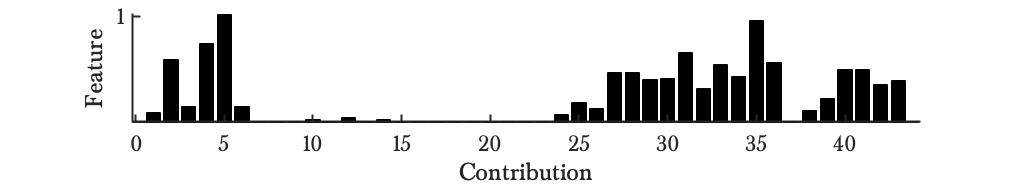
\includegraphics[width=.98\textwidth]{parts/chap-4/img-svm/pca-features-3.png}
            \caption{Mean of the 6 first PCA coefficients.} 
        \end{subfigure}
        \vfill
        \begin{subfigure}[b]{1\textwidth}   
            \centering 
            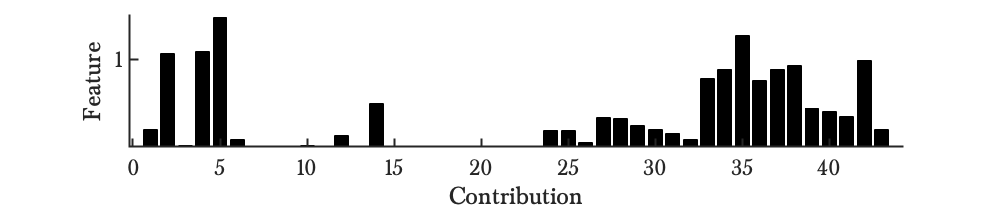
\includegraphics[width=.98\textwidth]{parts/chap-4/img-svm/pca-features-3-bis.png}
            \caption{Mean of the first 16 PCA coefficients.} 
        \end{subfigure}
        \vfill
        \begin{subfigure}[b]{1\textwidth}   
            \centering 
            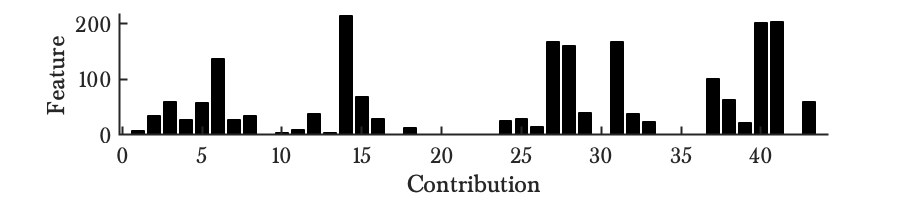
\includegraphics[width=.98\textwidth]{parts/chap-4/img-svm/chi2-features.png}
            \caption{Mean of the $\chi^2$ measure on all the model's SVMs.} 
        \end{subfigure}
        \caption{Evaluation of three different models in function of number of principal komponents kept. The one-against-all (or parallel) model is in dash-dotted line, the tree-bases model (or parallel) are the plain and dotted line. For the plain line, the order of the SVMs is \{Normal, DoS, Prob, R2L, U2R\} and the dotted line is \{Probe, U2R, R2L, DoS, Normal\}. Every result is the mean of 5 different experiments with different training and test sets.}
        \label{fig:features-part}
\end{figure}

A last thing, performing a $k$-means clustering algorithm isn't much interesting in the case of support vector machines as the sole parameter influencing the evaluation time are the support vectors, which are by essence of support vector machines, close to the decision boundary. The number of data-points far from the decision boundary --- which we try to reduce with a $k$-means algorithm --- have thus no influence on the number of support vectors. The eventual only gain of reducing the data-set size with a $k$-means algorithm is to reduce training time, but this is not much of our concern here.

\FloatBarrier
\subsubsection{Evaluation execution}
% TO BE DONE LATER

\subsection{Non-linear support vector machines}
Now that we have benchmarked the linear model, we can have a look at some non-linear models. Performing KPCA with linear support vector machines is not very relevant. Indeed, we should always prefer a support vector machine with radial based kernel functions. Both compute the kernel matrix, but compute the output in different manners. 
\begin{itemize}
    \item \textbf{KPCA-SVM} The KPCA will compute a linear combination very likely all $k(x_,x_i)$ and thus all input vectors $x_i$. Each new feature of the transformed data-points will be a linear combination of a radial based function with all the original training data-points of the KPCA. These linear combinations are independent of the classes and are general for the whole data-set. Whatever the number of chosen output features, the new data-point will have to be evaluated through $k(x_,x_i)$ against all original KPCA training data-points.
    \item \textbf{RBF-SVM} The big advantage of SVM with radial based kernel functions is that the kernel function is used in the SVM and not beforehand, independently of it. The results are thus better. Furthermore, the original training data-points against which a new query point are computed are limited to the number of support vectors, i.e. the ones critical to the boundary. This drastically diminishes their number and improves the evaluation time of a new query point.
\end{itemize}
However, some alternative methods use KPCA combined with linear SVMs in some clever way (KPCA-SVM) to approximate RBF-SVM and significantly decrease the training time, but augmenting the evaluation time. This is the opposite trade-off of the one we are looking for and we will thus not consider it.

Figure~\ref{fig:svm-nl} shows the results of a radial based function support vector machine on the NSL-KDD data-set. The box constraints $C$ and the kernel function parameter $\sigma^2$ are optimized at each specific training through a 10-fold cross-validation. 

A first observation compared to the linear support vector machines models is the much better accuracy. This is due to the added non-linearity which allows more complexity. The individual scores of the support vector machines are attaining values very close to 100\%. We can observe that accuracy and Cohen's kappa coefficient are following almost exactly the same graph, at the difference of a factor. This is typical when the models are attaining very high accuracies and make little mistakes. This comforts us in our claim of a good model.

A second observation is the same we made here before with the linear support vector machines: the tree-based model are performing worse than the one-against-all model. Here again, the accuracy doesn't increase much more after $n=15,000$. A difference with before is the better performance of the other sequence of the tree-based model, even though the difference is minimal. Results for the best tree-based model and the one-against-all model are given in tables~\ref{tab:svm-nl-0} and \ref{tab:svm-nl-1}. As we can see, the errors are marginal and $n=50,000$ doesn't add a lot of improvement.

\begin{figure}
        \begin{subfigure}[b]{1\textwidth}  
            \centering 
            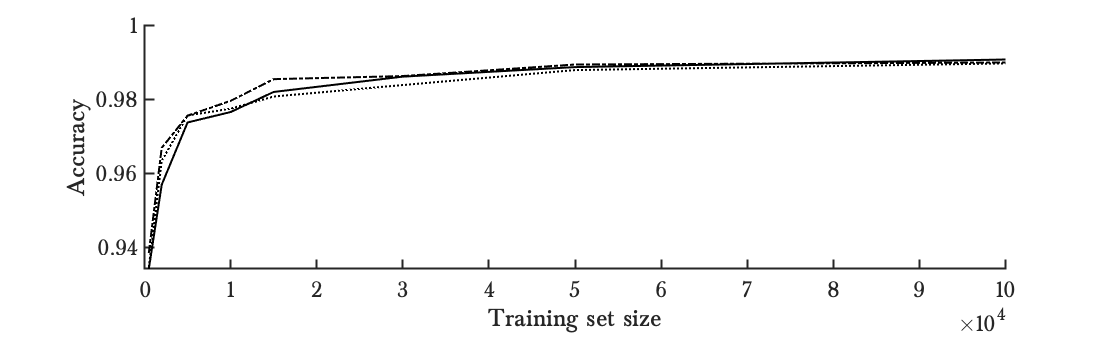
\includegraphics[width=.98\textwidth]{parts/chap-4/img-svm/svm-nl-acc.png}
            \caption{Mean Accuracy on the test set.} 
        \end{subfigure}
        \vfill
        \begin{subfigure}[b]{1\textwidth}   
            \centering 
            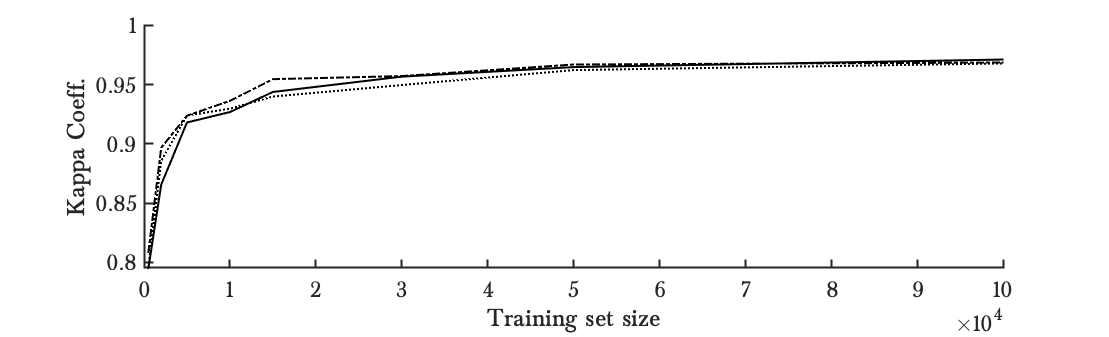
\includegraphics[width=.98\textwidth]{parts/chap-4/img-svm/svm-nl-kappa.png}
            \caption{Mean Cohen's kappa coefficient.} 
        \end{subfigure}
        \caption{Evaluation of three different models in function of the training set size. The one-against-all (or parallel) model is in dash-dotted line, the tree-bases model (or parallel) are the plain and dotted line. For the plain line, the order of the SVMs is \{Normal, DoS, Prob, R2L, U2R\} and the dotted line is \{Probe, U2R, R2L, DoS, Normal\}. Every result is the mean of 5 different experiments with different training and test set.}
        \label{fig:svm-nl}
\end{figure}

\begin{table}[ht!]
    \centering
    \begin{tabularx}{\textwidth}{lcccccc}
    \hlineI
    Model & Normal & Probe & Dos & R2L & U2R & Total \\ \hlineI
    \textbf{Tree 1} with $n=15,000$ & & & & & &\\
    Accuracy [\%] & 97.82 & 99.08 & 99.01 & 91.71 & 24.00 & 98.20\\ 
    MCC & 96.62 & 99.03 & 98.54 & 87.47 & 32.25 & 82.78\\ 
    Kappa & 23.65 & 42.23 & 42.14 & 93.71 & 99.69 & 94.39\\  \hline
    Obs. Normal  & 2935 & 7 & 21 & 33 & 5 & \\ 
    Obs. Probe  & 18 & 2229 & 2 & 0 & 0 & \\ 
    Obs. DoS  & 19 & 2 & 2228 & 1 & 0 & \\ 
    Obs. R2L  & 16 & 1 & 1 & 215 & 1 & \\ 
    Obs. U2R  & 5 & 0 & 0 & 6 & 4 & \\   \hlineI
    
    \textbf{Tree 2} with $n=15,000$ & & & & & &\\
    Accuracy [\%] & 97.98 & 98.25 & 99.20 & 91.45 & 28.00 & 98.08\\ 
    MCC & 96.23 & 98.44 & 98.56 & 89.30 & $\emptyset$ & $\emptyset$\\ 
    Kappa & 23.46 & 42.56 & 42.04 & 93.85 & 99.72 & 94.00\\  \hline
    Obs. Normal  & 2939 & 8 & 24 & 26 & 2 & \\ 
    Obs. Probe  & 36 & 2211 & 4 & 0 & 0 & \\ 
    Obs. DoS  & 17 & 1 & 2232 & 0 & 0 & \\ 
    Obs. R2L  & 19 & 1 & 0 & 214 & 0 & \\ 
    Obs. U2R  & 7 & 0 & 0 & 3 & 4 & \\  \hlineI
    
    \textbf{O-A-A} with $n=15,000$ & & & & & &\\
    Accuracy [\%] & 98.33 & 99.40 & 99.15 & 92.14 & 24.00 & 98.55\\ 
    MCC & 97.28 & 99.41 & 98.84 & 88.54 & 33.55 & 83.52\\ 
    Kappa & 23.38 & 42.13 & 42.14 & 93.76 & 99.72 & 95.47\\   \hline 
    Obs. Normal  & 2950 & 4 & 15 & 30 & 1 & \\ 
    Obs. Probe  & 12 & 2237 & 1 & 0 & 0 & \\ 
    Obs. DoS  & 18 & 1 & 2231 & 0 & 0 & \\ 
    Obs. R2L  & 15 & 1 & 0 & 216 & 2 & \\ 
    Obs. U2R  & 5 & 0 & 1 & 5 & 4 & \\ \hlineI
    \end{tabularx}
    \caption{Detailed results of the $k$-NN classification algorithm for two different values of the number of neighbours $k$ and for a big and a small training data-set. The accuracy, true positive rate (TP), true negative rate (TN), false positive rate (FP) and false negative rate (FN) are given for each target class.}
    \label{tab:svm-nl-0}
\end{table}

\begin{table}[ht!]
    \centering
    \begin{tabularx}{\textwidth}{lcccccc}
    \hlineI
    Model & Normal & Probe & Dos & R2L & U2R & Total \\ \hlineI
    \textbf{Tree 1} with $n=50,000$ & & & & & &\\
    Accuracy [\%] & 98.79 & 99.38 & 99.32 & 92.35 & 35.56 & 98.88\\ 
    MCC [\%] & 97.82 & 99.42 & 98.98 & 91.23 & 48.81 & 87.25\\ 
    Kappa [\%] & 23.00 & 41.75 & 41.68 & 94.69 & 99.82 & 96.46\\  \hline
    Obs. Normal  & 2964 & 3 & 16 & 16 & 1 & \\ 
    Obs. Probe  & 13 & 2248 & 1 & 0 & 0 & \\ 
    Obs. DoS  & 13 & 2 & 2247 & 0 & 0 & \\ 
    Obs. R2L  & 15 & 0 & 0 & 188 & 1 & \\ 
    Obs. U2R  & 3 & 0 & 0 & 3 & 3 & \\  \hlineI
    
    \textbf{Tree 2} with $n=50,000$ & & & & & &\\
    Accuracy [\%] & 98.93 & 99.02 & 99.27 & 91.76 & 40.00 & 98.80\\ 
    MCC [\%] & 97.57 & 99.14 & 98.99 & 92.25 & 53.45 & 88.28\\ 
    Kappa [\%] & 22.86 & 41.89 & 41.71 & 94.78 & 99.82 & 96.24\\   \hline
    Obs. Normal  & 2968 & 5 & 15 & 12 & 1 & \\ 
    Obs. Probe  & 22 & 2240 & 1 & 0 & 0 & \\ 
    Obs. DoS  & 16 & 0 & 2245 & 0 & 0 & \\ 
    Obs. R2L  & 16 & 0 & 0 & 187 & 1 & \\ 
    Obs. U2R  & 3 & 0 & 0 & 2 & 4 & \\   \hlineI
    
    \textbf{O-A-A} with $n=50,000$ & & & & & &\\
    Accuracy [\%] & 98.80 & 99.59 & 99.37 & 91.86 & 37.78 & 98.95\\ 
    MCC [\%] & 97.94 & 99.61 & 99.03 & 91.09 & 45.08 & 86.55\\ 
    Kappa [\%] & 23.02 & 41.67 & 41.66 & 94.71 & 99.81 & 96.70\\   \hline
    Obs. Normal  & 2964 & 3 & 16 & 16 & 1 & \\ 
    Obs. Probe  & 8 & 2253 & 1 & 0 & 0 & \\ 
    Obs. DoS  & 13 & 1 & 2248 & 0 & 0 & \\ 
    Obs. R2L  & 15 & 0 & 0 & 187 & 1 & \\ 
    Obs. U2R  & 3 & 0 & 0 & 2 & 3 & \\  \hlineI
    \end{tabularx}
    \caption{Detailed results of the $k$-NN classification algorithm for two different values of the number of neighbours $k$ and for a big and a small training data-set. The accuracy, true positive rate (TP), true negative rate (TN), false positive rate (FP) and false negative rate (FN) are given for each target class.}
    \label{tab:svm-nl-1}
\end{table}

Figure~\ref{} shows how much time each of these classifiers take to evaluate a single test point. 
% TO BE DONE LATER

\FloatBarrier
\subsubsection{Support vector reduction}
A difference with linear support vector machines though is that the use of a kernel matrix doesn't allow us to evaluate a new data-point in the primal space anymore. This primal space had the dimension of the feature space and the training size had not a lot of influence on the evaluation of a new query point as a consequence. However, this is not the case anymore and the evaluation now happens in a support vector space. As a reminder, the evaluation of a new data-point $x$ in the SVM now is given by
\begin{equation}
    \sum_{i=1}^{n_{sv}} \alpha_i l_k k(x,x_i)
\end{equation}
where $k(x,x_i)$ is the kernel function and $n_sv$ the number of support vectors. For each of our models trained before, the number of support vectors is given at figure~\ref{fig:svm-nl-sv}. The number of support vectors is much higher for the one-against-all model as suspected as it has one more support vector machine than the tree-based model. However, an interesting observation is that both tree-based models --- although having the same number number of support vector machines --- have a significant divergence in the total number of support vectors. Furthermore, it is the best of both models that comprises the less number of support vectors. In this latter case, the total number of support vectors never exceeds significantly a thousand. Let's however see if we can reduce this number further.

\begin{figure}[ht!]
    \centering
    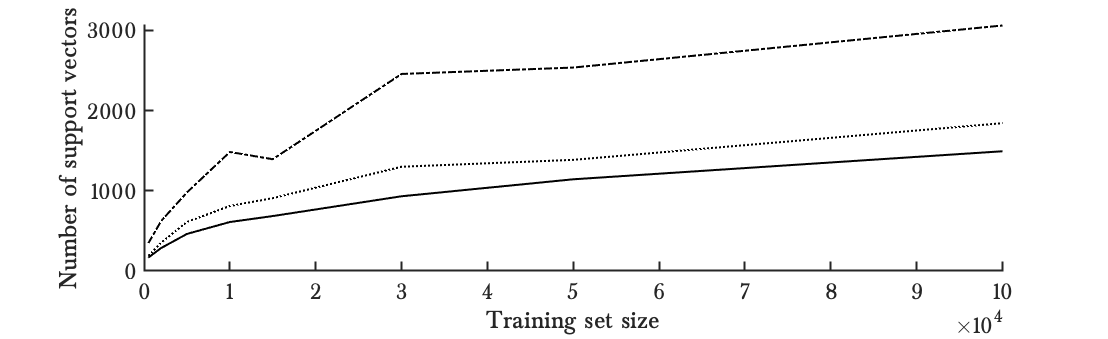
\includegraphics[width=1\textwidth]{parts/chap-4/img-svm/svm-nl-sv.png}
    \caption{Total number of support vectors for different models based on the training set size. The one-against-all (or parallel) model is in dash-dotted line, the tree-bases model (or parallel) are the plain and dotted line. For the plain line, the order of the SVMs is \{Normal, DoS, Prob, R2L, U2R\} and the dotted line is \{Probe, U2R, R2L, DoS, Normal\}. Every result is the mean of 5 different experiments with different training and test set.}
    \label{fig:svm-nl-sv}
\end{figure}

As we said before, $C$ is optimized through validation. This directly controls the number of support vectors. To improve the speed of the evaluation, one must thus reduce the number of support vectors. This can be controlled by the box constraint $C$ which --- as a reminder --- represents the trade-off between the objective of a support vector machine and the influence of the slack variables --- we could the corresponding data-points the "difficult" ones. In this sense, a high value of $C$ will just make the boundary absolutely fit to every variable and tolerate no wrongly classified data-point to the model. In other words, the difficult data-points will have a much higher influence. This is even more clear in the dual as the box constraint $C$ directly represents an upper bound on the $\alpha_i$. A high value of $C$ leads to less regularization and the model to fit to these specific difficult points, which increases the risk of overfitting. Let's investigate how far we can increase the box constraint $C$ without suffering from overfitting. By this mean, we can reduce the MPC evaluation without having too much impact on the accuracy.

Figure~\ref{fig:svm-nl-red} shows how the number of support vector decreases as the box constraint parameter $C$ increases. The result of the last SVM shows more variability as the low number of data-points of the classes R2L and U2R which it classifies. In general, we can observe that the after a certain value, the number of support vectors doesn't decrease anymore and the accuracy, which is almost perfect stagnates. However, we see that we aren't really subject to overfitting. The stagnation of the number of support vectors and the absence of ovefitting tells us that all data-points are within the good side of the boundary. In this sense, imposing the missclassified ones to fit to the boundary has no effect, hence the stagnation. In a certain sense, this corresponds to the ideal boundary. However, the very high box constraint $C$ also diminishes the impact of the first term of the boundary, which controls the smoothening of the boundary. However, finding the optimal $C$ without imposing it to be high already naturally tends a high value. This indicates that the optimal boundary without the constraint of lowering the number of support vectors is not smooth. In this sense, the boundary is only defined by the critical data-points. These sole critical data-points are the only one the support vectors consists of. This is also the reason for the stagnation of their number.

\begin{figure}[ht!]
        \begin{subfigure}[b]{.47\textwidth}  
            \centering 
            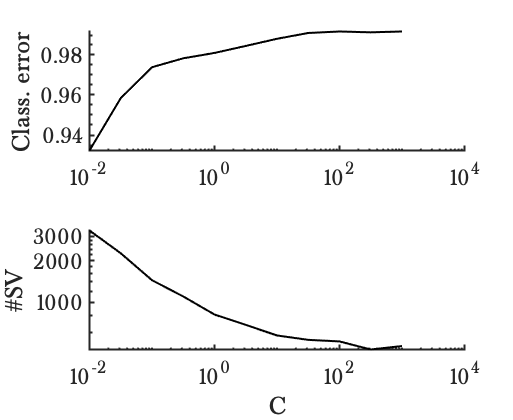
\includegraphics[width=.98\textwidth]{parts/chap-4/img-svm/non-lin/svm1.png}
            \caption{First SVM.} 
        \end{subfigure}
        \hfill
        \begin{subfigure}[b]{.47\textwidth}   
            \centering 
            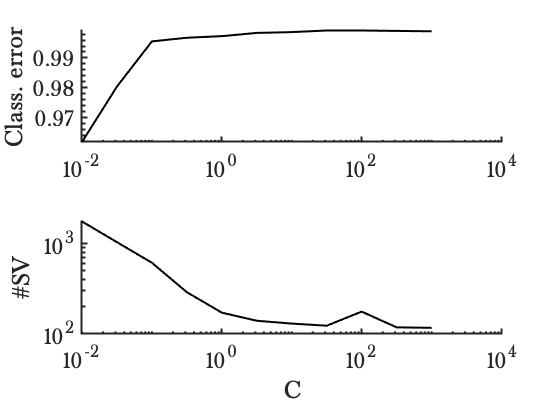
\includegraphics[width=.98\textwidth]{parts/chap-4/img-svm/non-lin/svm2.png}
            \caption{Second SVM.} 
        \end{subfigure}
        \hfill
        \begin{subfigure}[b]{.47\textwidth}   
            \centering 
            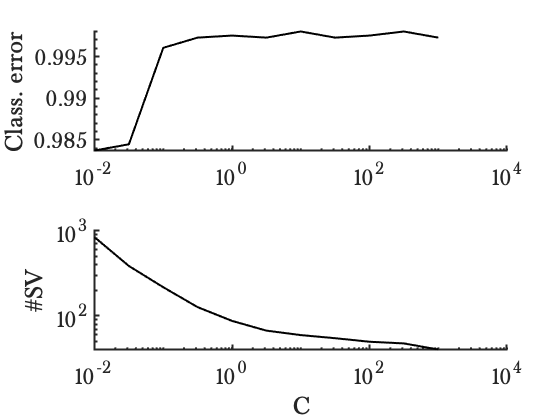
\includegraphics[width=.98\textwidth]{parts/chap-4/img-svm/non-lin/svm3.png}
            \caption{Third SVM.} 
        \end{subfigure}
        \hfill
        \begin{subfigure}[b]{.47\textwidth}   
            \centering 
            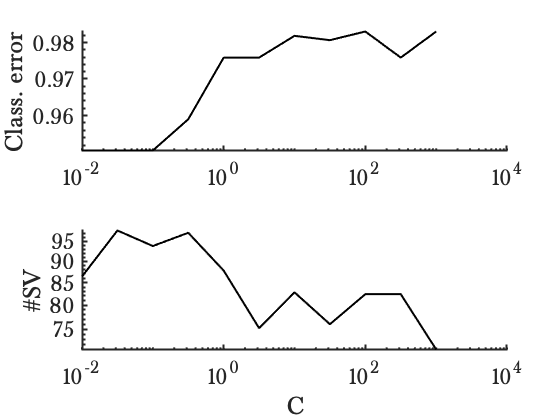
\includegraphics[width=.98\textwidth]{parts/chap-4/img-svm/non-lin/svm4.png}
            \caption{Fourth SVM.} 
        \end{subfigure}
        \caption{Support vector reduction for the tree-based model with SVM order \{Normal, DoS, Prob, R2L, U2R\} with $n=15,000$ data-points.}
        \label{fig:svm-nl-red}
\end{figure}

By taking a very high value of $C$ to reduce the number of support vectors, we still obtain a similar accuracy as before (table~\ref{}. However the number of support vectors went from 931 with the classically validated $C$ to 588 with a high value of $C$. This is decrease of 37\% and we can expect a similar increase in time. For the other tree-based model, the number of support vectors went from 908 to 643 representing a decrease of 29\% For the one-against-all model, it went from 1393 to 1031 representing a decrease of 35\%.

\begin{table}[ht!]
    \centering
    \begin{tabularx}{\textwidth}{lcccccccc}
    \hlineI
    Model &&& Normal & Probe & Dos & R2L & U2R & Total \\ \hlineI
    \multicolumn{9}{l}{\textbf{Tree 1} with $n=15,000$ and support vector reduction}\\
    Accuracy [\%] &&& 98.61 & 99.71 & 98.98 & 93.76 & 52 & 98.84\\ 
    MCC &&& 97.88 & 99.57 & 98.83 & 91.01 & 45.04 & 86.47\\ 
    Kappa &&& 23.21 & 41.79 & 42.04 & 94.15 & 99.72 & 96.37\\   \hline
    Obs. Normal  &&& 2958 & 5 & 13 & 21 & 3 & \\ 
    Obs. Probe  &&& 4 & 2249 & 1 & 1 & 1 & \\ 
    Obs. DoS  &&& 20 & 2 & 2233 & 1 & 0 & \\ 
    Obs. R2L  &&& 11 & 0 & 0 & 207 & 3 & \\ 
    Obs. U2R  &&& 1 & 0 & 0 & 4 & 5 & \\   \hlineI
    
    \multicolumn{9}{l}{\textbf{Tree 2} with $n=15,000$ and support vector reduction}\\
    Accuracy [\%] &&& 98.69 & 99.71 & 99.25 & 90.77 & 74 & 98.89\\ 
    MCC &&& 97.93 & 99.51 & 99.00 & 90.79 & 63.39 & 90.13\\ 
    Kappa &&& 23.16 & 41.78 & 41.92 & 94.32 & 99.70 & 96.54 \\ \hline
    Obs. Normal  &&& 2961 & 7 & 11 & 18 & 4 & \\ 
    Obs. Probe && & 3 & 2249 & 4 & 0 & 0 & \\ 
    Obs. DoS && & 16 & 1 & 2239 & 0 & 0 & \\ 
    Obs. R2L && & 17 & 1 & 0 & 201 & 2 & \\ 
    Obs. U2R && & 2 & 0 & 0 & 1 & 7 & \\  \hlineI
    
     \multicolumn{9}{l}{\textbf{O-A-A} with $n=15,000$ and support vector reduction}\\
    Accuracy [\%] &&& 98.72 & 99.69 & 99.34 & 92.04 & 74 & 98.96\\ 
    MCC &&& 98.07 & 99.61 & 98.98 & 91.60 & 63.42 & 90.34\\ 
    Kappa &&& 23.16 & 41.81 & 41.87 & 94.29 & 99.69 & 96.75\\    \hline 
    Obs. Normal && & 2962 & 4 & 13 & 17 & 4 & \\ 
    Obs. Probe && & 4 & 2249 & 3 & 0 & 0 & \\ 
    Obs. DoS && & 14 & 1 & 2241 & 0 & 0 & \\ 
    Obs. R2L && & 14 & 0 & 1 & 203 & 2 & \\ 
    Obs. U2R && & 1 & 0 & 1 & 1 & 7 & \\  \hlineI
    \end{tabularx}
    \caption{Detailed results of the $k$-NN classification algorithm for two different values of the number of neighbours $k$ and for a big and a small training data-set. The accuracy, true positive rate (TP), true negative rate (TN), false positive rate (FP) and false negative rate (FN) are given for each target class.}
    \label{tab:svm-nl-0}
\end{table}

\FloatBarrier

\subsubsection{PCA with support vector reduction}
Each tested data-point has to be computed against all support vectors. Now that the number of support vectors has been reduced, let us investigate if we can also reduce the evaluation of each support vector in itself. As a reminder, the radial based kernel function is given by
\begin{equation}
    k(x,y) = e^{\frac{\norm{x-y}^2}{2\sigma^2}}
\end{equation}
and the norm is given by
\begin{equation}
    \norm{x-y} = \sum_{j=1}^{d} (x_j - y_j)^2
\end{equation}
where $d$ is the number of features.

By applying a PCA decomposition, we would be able to approximate the norm and limit the sum to $n_{pca}$ terms instead of $d$ terms. The evaluation against each support vector would then be reduced. The cost of doing this is the need to transform each tested data-point through PCA. As we saw before this evaluation is of complexity $\mathcal{O}(n_{pca}d)$. In the contrary as before, this is far smaller than the complexity needed to evaluate the SVM due to the much higher number of support vectors. The need for evaluating one of the two in clear is thus not justified anymore. Indeed, evaluating the SVM-part in clear would reveal the feature vectors which are highly sensitive data and the evaluation of the PCA-part in clear is significantly less costly than the SVM. We will thus only interest us in evaluating the whole (PCA and SVM) in MPC.

Furthermore, the norm in the feature space gives the same weight to each feature. Using a PCA decomposition will vary the weight. \noteH{maybe more explanation, but this requires a lot.} 

Results of the PCA decomposition with RBF-SVM are given at figure~\ref{fig:svm-nl-pca}. In comparison to the PCA transformation with linear support vector machines, a lower number of principal components kept is here feasible (8 gave not satsifying results with the SVMs with linear kernel, and seems here satisfying). A low number of principal components seems also to impose a higher number of support vectors. This makes sense as the more information lost during the PCA transformation has to be compensated by keeping more information in the SVM under the form of support vectors. Table~\ref{tab:svm-nl-pca} shows the results with 16 principal components. We can clearly see that the performance is as good as without any PCA reduction.

\begin{figure}[ht!]
        \begin{subfigure}[b]{.97\textwidth}  
            \centering 
            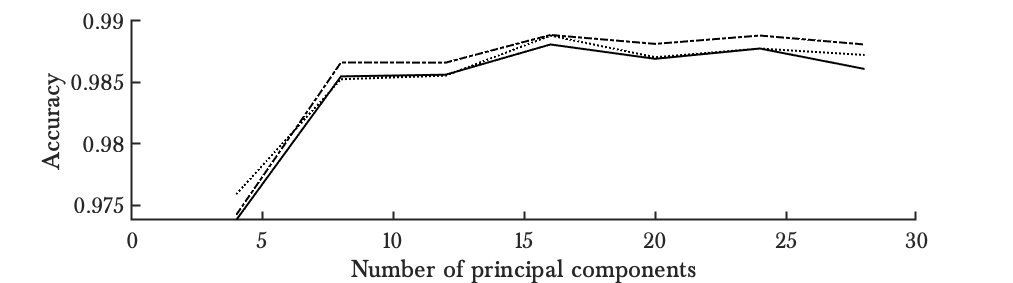
\includegraphics[width=.98\textwidth]{parts/chap-4/img-svm/nl-pca/acc.png}
            \caption{Accuracy in function of the number of principal components.} 
        \end{subfigure}
        \vfill
        \begin{subfigure}[b]{.97\textwidth}  
            \centering 
            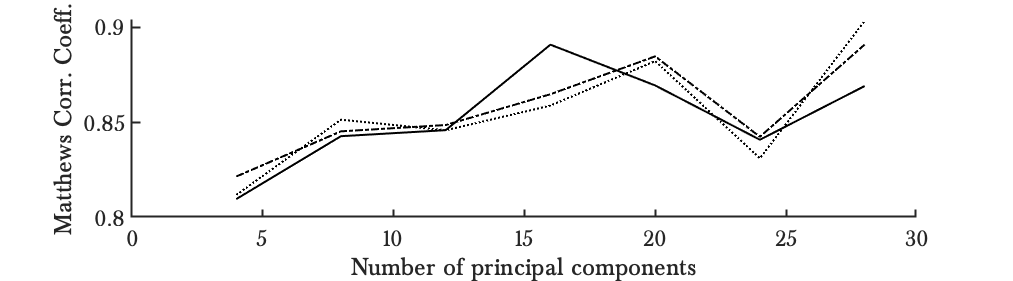
\includegraphics[width=.98\textwidth]{parts/chap-4/img-svm/nl-pca/mcc.png}
            \caption{Matthews correlation coefficient in function of the number of principal components.} 
        \end{subfigure}
        \vfill
        \begin{subfigure}[b]{.97\textwidth}  
            \centering 
            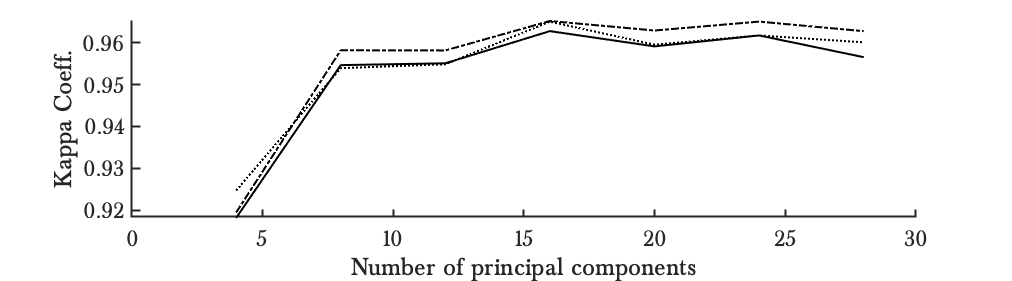
\includegraphics[width=.98\textwidth]{parts/chap-4/img-svm/nl-pca/kappa.png}
            \caption{Cohen's kappa coefficient in function of the number of principal components.} 
        \end{subfigure}
        \begin{subfigure}[b]{.97\textwidth}  
            \centering 
            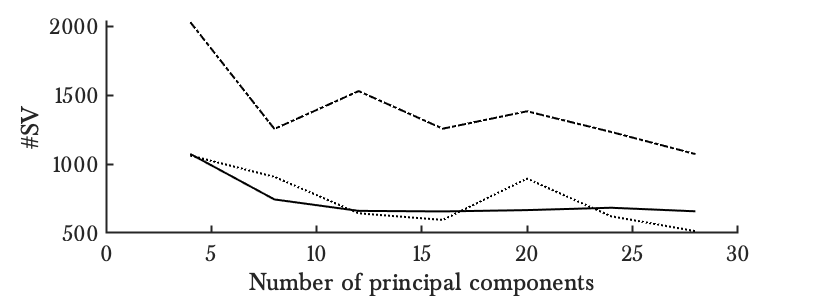
\includegraphics[width=.98\textwidth]{parts/chap-4/img-svm/nl-pca/sv.png}
            \caption{Total number of support vectors in function of the number of principal components.} 
        \end{subfigure}
        \caption{Influence of the number of principal components kept in a RBF-SVM with support with support vector reduction. The one-against-all (or parallel) model is in dash-dotted line, the tree-bases model (or parallel) are the plain and dotted line. For the plain line, the order of the SVMs is \{Normal, DoS, Prob, R2L, U2R\} and the dotted line is \{Probe, U2R, R2L, DoS, Normal\}. Every result is the mean of 5 different experiments with different training and test set.}
        \label{fig:svm-nl-pca}
\end{figure}

\begin{table}[ht!]
    \centering
    \begin{tabularx}{\textwidth}{lcccccccc}
    \hlineI
    Model &&& Normal & Probe & Dos & R2L & U2R & Total \\ \hlineI
    \multicolumn{9}{l}{\textbf{Tree 1} with $n=15,000$, $n_{pca}=16$ and support vector reduction}\\
    Accuracy [\%] &&& 98.31 & 99.55 & 99.00 & 97.40 & 54.29 & 98.81\\ 
    MCC [\%] &&& 97.74 & 99.42 & 98.65 & 92.45 & 57.14 & 89.08\\ 
    Kappa [\%] &&& 23.38 & 41.75 & 41.88 & 94.17 & 99.83 & 96.28\\   \hline
    Obs. Normal  &&& 2949 & 7 & 17 & 23 & 3 & \\ 
    Obs. Probe  &&& 4 & 2249 & 3 & 3 & 0 & \\ 
    Obs. DoS  &&& 20 & 1 & 2236 & 2 & 0 & \\ 
    Obs. R2L  &&& 5 & 0 & 0 & 209 & 0 & \\ 
    Obs. U2R  &&& 3 & 0 & 0 & 1 & 4 & \\  \hlineI
    
    \multicolumn{9}{l}{\textbf{Tree 2} with $n=15,000$, $n_{pca}=16$ and support vector reduction}\\
    Accuracy [\%] &&& 98.44 & 99.65 & 99.11 & 96.28 & 45.71 & 98.88\\ 
    MCC [\%]  &&& 97.87 & 99.47 & 98.76 & 93.62 & 39.74 & 85.89\\ 
    Kappa [\%] &&& 23.31 & 41.70 & 41.85 & 94.30 & 99.78 & 96.50\\  \hline
    Obs. Normal  &&& 2953 & 6 & 17 & 18 & 6 & \\ 
    Obs. Probe && & 4 & 2251 & 2 & 2 & 0 & \\ 
    Obs. DoS && & 16 & 3 & 2239 & 0 & 1 & \\ 
    Obs. R2L && & 8 & 0 & 0 & 207 & 0 & \\ 
    Obs. U2R && & 3 & 0 & 0 & 0 & 3 & \\  \hlineI
    
     \multicolumn{9}{l}{\textbf{O-A-A} with $n=15,000$, $n_{pca}=16$ and support vector reduction}\\
    Accuracy [\%] &&& 98.58 & 99.64 & 99.01 & 95.72 & 45.71 & 98.89\\ 
    MCC [\%] &&& 97.83 & 99.56 & 98.71 & 93.47 & 42.85 & 86.48\\ 
    Kappa [\%] &&& 23.20 & 41.73 & 41.89 & 94.33 & 99.80 & 96.52\\    \hline 
    Obs. Normal && & 2957 & 5 & 16 & 16 & 6 & \\ 
    Obs. Probe && & 4 & 2251 & 3 & 1 & 0 & \\ 
    Obs. DoS && & 21 & 1 & 2237 & 1 & 0 & \\ 
    Obs. R2L && & 9 & 0 & 0 & 206 & 0 & \\ 
    Obs. U2R && & 4 & 0 & 0 & 0 & 3 & \\  \hlineI
    \end{tabularx}
    \caption{Detailed results of the $k$-NN classification algorithm for two different values of the number of neighbours $k$ and for a big and a small training data-set. The accuracy, true positive rate (TP), true negative rate (TN), false positive rate (FP) and false negative rate (FN) are given for each target class.}
    \label{tab:svm-nl-pca}
\end{table}

\FloatBarrier
\subsubsection{$\chi^2$ with support vector reduction}
Similarly, to limit the number of terms in the sum needed for the norm, we could also perform a $\chi^2$ feature selection as we did before. Computing the selected features with radial based kernel function support vector machines gives very similar results as with the linear one. However, although both methods are keeping 33 of the 43 features, these are not exactly the same. This indicates that some features have a more linear impact on the output and some others have a more local impact. However, apart from a few exceptions, the kept inputs are the same indicating their clear contribution however this contribution is taken into account. Figure~\ref{fig:svm-nl-chi2} shows the $\chi^2$ measure of each SVM of a tree-based model. It is very clear that the model with few training data obtains much lower scores.

Another detail is that a feasible cut-off value on the $\chi^2$ measure with RBF-SVM is much higher than with linear SVMs. This indicates that the correspondig certainty\footnote{The $\chi^2$ measure used here is based on the classical $\chi^2$ test for categorical data which uses a p-value relevance estimation. Here, we cannot use this test directly as we don't have categrocial data as feature inputs. In a certain sense, for each of our tests on each support vector machine, we have 4 input classes used (TP, TN, FP, FN) and two output classes (1 or 0). This corresponds to a $\chi^2$ with three degrees of freedom. The cut-off value chosen here (10) corresponds to a p-value of .018566. This is statistically satisfying. However, this is not the goal we pursue here. The only thing that matters is finding clever ways to improve the speed of the evaluation of a test-set through our MPC models. For the linear based SVM, the p-value was not satisfying (p > 0.5). However, it still allowed us to improve the speed without loosing in accuracy.} is much higher. But the most interesting part is that here again, reducing the number of feature inputs by pure selection allows us to keep the same high performance while reducing the model's complexity and evaluation time (table~\ref{tab:svm-nl-chi2}).

\begin{figure}[ht!]
        \begin{subfigure}[b]{.97\textwidth}  
            \centering 
            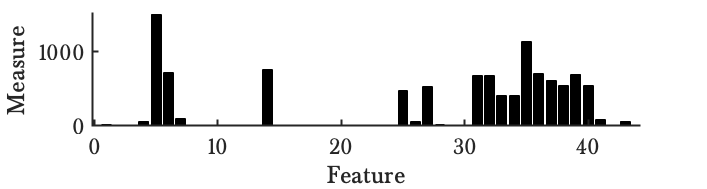
\includegraphics[width=.98\textwidth]{parts/chap-4/img-svm/nl-chi2/svm3.png}
            \caption{First SVM of the model.} 
        \end{subfigure}
        \vfill
         \begin{subfigure}[b]{.97\textwidth}  
            \centering 
            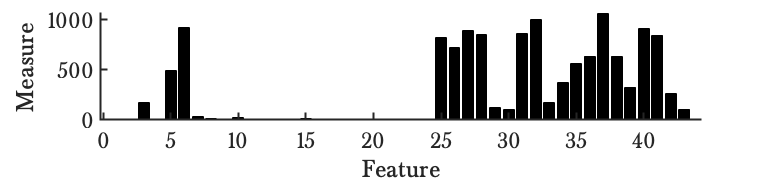
\includegraphics[width=.98\textwidth]{parts/chap-4/img-svm/nl-chi2/svm2.png}
            \caption{Second SVM of the model.} 
        \end{subfigure}
        \vfill
         \begin{subfigure}[b]{.97\textwidth}  
            \centering 
            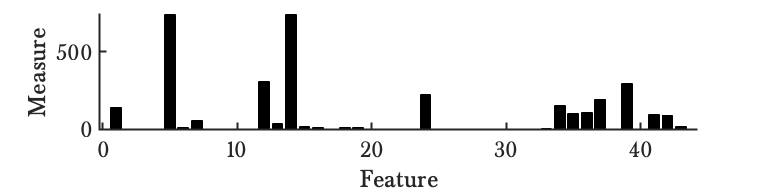
\includegraphics[width=.98\textwidth]{parts/chap-4/img-svm/nl-chi2/svm4.png}
            \caption{Third SVM of the model.} 
        \end{subfigure}
        \vfill
         \begin{subfigure}[b]{.97\textwidth}  
            \centering 
            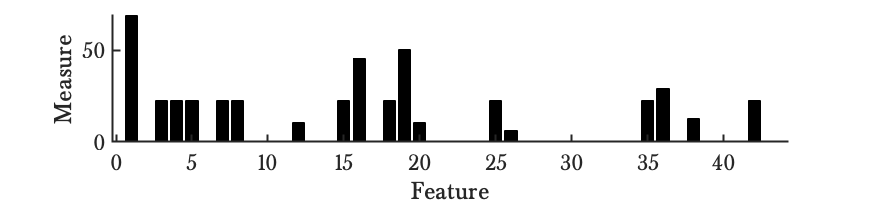
\includegraphics[width=.98\textwidth]{parts/chap-4/img-svm/nl-chi2/svm1.png}
            \caption{Fourth SVM of the model.} 
        \end{subfigure}
        \caption{$\chi^2$ measure for each feature in each SVM of the tree-based model with order \{Normal, DoS, Prob, R2L, U2R\}.}
        \label{fig:svm-nl-chi2}
\end{figure}

\begin{table}[ht!]
    \centering
    \begin{tabularx}{\textwidth}{lcccccccc}
    \hlineI
    Model &&& Normal & Probe & Dos & R2L & U2R & Total \\ \hlineI
    \multicolumn{9}{l}{\textbf{Tree 1} with $n=15,000$, $n_{pca}=16$ and support vector reduction}\\
    Accuracy [\%] &&& 98.24 & 99.49 & 99.02 & 95.95 & 43.08 & 98.67\\ 
    MCC [\%] &&& 97.47 & 99.43 & 98.60 & 91.35 & 53.68 & 88.11\\ 
    Kappa [\%] &&& 23.44 & 41.92 & 42.00 & 94.00 & 99.73 & 95.85\\   \hline
    Obs. Normal  &&& 2947 & 5 & 20 & 25 & 2 & \\ 
    Obs. Probe  &&& 9 & 2244 & 2 & 0 & 0 & \\ 
    Obs. DoS  &&& 20 & 1 & 2233 & 1 & 0 & \\ 
    Obs. R2L  &&& 8 & 0 & 0 & 213 & 0 & \\ 
    Obs. U2R  &&& 3 & 0 & 0 & 4 & 6 & \\  \hlineI
    
    \multicolumn{9}{l}{\textbf{Tree 2} with $n=15,000$, $n_{pca}=16$ and support vector reduction}\\
    Accuracy [\%] &&& 98.55 & 99.74 & 99.14 & 94.14 & 56.92 & 98.87\\ 
    MCC [\%]  &&& 97.76 & 99.54 & 98.75 & 93.76 & 60.11 & 89.98\\ 
    Kappa [\%] &&& 23.25 & 41.81 & 41.96 & 94.26 & 99.67 & 96.48\\   \hline
    Obs. Normal  &&& 2957 & 6 & 19 & 14 & 5 & \\ 
    Obs. Probe && & 4 & 2249 & 2 & 0 & 0 & \\ 
    Obs. DoS && & 18 & 1 & 2236 & 0 & 0 & \\ 
    Obs. R2L && & 12 & 1 & 0 & 209 & 0 & \\ 
    Obs. U2R && & 6 & 0 & 0 & 0 & 7 & \\ \hlineI
    
     \multicolumn{9}{l}{\textbf{O-A-A} with $n=15,000$, $n_{pca}=16$ and support vector reduction}\\
    Accuracy [\%] &&& 98.54 & 99.73 & 99.16 & 94.14 & 61.54 & 98.88\\ 
    MCC [\%] &&& 97.81 & 99.62 & 98.79 & 92.57 & 62.34 & 90.23\\ 
    Kappa [\%] &&& 23.27 & 41.83 & 41.96 & 94.19 & 99.67 & 96.50\\    \hline 
    Obs. Normal && & 2956 & 4 & 17 & 19 & 4 & \\ 
    Obs. Probe && & 4 & 2249 & 1 & 0 & 0 & \\ 
    Obs. DoS && & 17 & 1 & 2236 & 0 & 0 & \\ 
    Obs. R2L && & 11 & 1 & 2 & 209 & 0 & \\ 
    Obs. U2R && & 5 & 0 & 0 & 0 & 8 & \\  \hlineI
    \end{tabularx}
    \caption{Detailed results of the $k$-NN classification algorithm for two different values of the number of neighbours $k$ and for a big and a small training data-set. The accuracy, true positive rate (TP), true negative rate (TN), false positive rate (FP) and false negative rate (FN) are given for each target class.}
    \label{tab:svm-nl-chi2}
\end{table}

\subsubsection{Time evaluation}


\FloatBarrier